
%%--------------------------------------------------
%% CPO: Multiple Choice Questions
%%--------------------------------------------------


%% Chapter 19: Harmonic Motion
%%--------------------------------------------------


%% Learning Objectives
%%--------------------------------------------------

%% Identify a cycle of harmonic motion. 
%% Recognize common oscillators. 
%% Know the relationship between period and frequency. 
%% Understand how to identify and measure amplitude. 
%% Recognize the difference between linear motion and harmonic motion graphs. 
%% Interpret graphs of harmonic motion. 
%% Determine amplitude and period from a harmonic motion graph. 
%% Recognize when two oscillators are in phase or out of phase. 
%% Understand the role of restoring force in how oscillators work. 
%% Learn the relationship between amplitude and period for a pendulum. 
%% Recognize simple oscillators.


%% CPO Multiple Choice Questions
%%--------------------------------------------------
\element{cpo-mc}{
\begin{question}{cpo-ch19-q01}
    Motion that occurs in repeated cycles includes all of the following \emph{except}:
    \begin{multicols}{2}
    \begin{choices}
        \wrongchoice{pendulum motion}
        \wrongchoice{harmonic motion}
      \correctchoice{linear motion}
        \wrongchoice{circular motion}
    \end{choices}
    \end{multicols}
\end{question}
}

\element{cpo-mc}{
\begin{question}{cpo-ch19-q02}
    A unit of motion repeated over and over again is called the:
    \begin{multicols}{2}
    \begin{choices}
        \wrongchoice{amplitude}
      \correctchoice{cycle}
        \wrongchoice{velocity}
        \wrongchoice{period}
    \end{choices}
    \end{multicols}
\end{question}
}

\element{cpo-mc}{
\begin{question}{cpo-ch19-q03}
    Oscillating systems include all of the following \emph{except}:
    \begin{choices}
        \wrongchoice{the moving pedals on a bicycle.}
        \wrongchoice{a radio signal from FM station 106.3.}
        \wrongchoice{Earth turning on its axis.}
      \correctchoice{a block sliding down a ramp.}
    \end{choices}
\end{question}
}

\element{cpo-mc}{
\begin{question}{cpo-ch19-q04}
    The measure of the number of cycles per second is called:
    \begin{multicols}{2}
    \begin{choices}
      \correctchoice{frequency}
        \wrongchoice{period}
        \wrongchoice{amplitude}
        \wrongchoice{vibration}
    \end{choices}
    \end{multicols}
\end{question}
}

\element{cpo-mc}{
\begin{question}{cpo-ch19-q05}
    The unit for measuring the frequency of an oscillating system is the:
    \begin{choices}
        \wrongchoice{meter (\si{\meter})}
        \wrongchoice{meter per second (\si{\meter\per\second})}
      \correctchoice{hertz (\si{\hertz})}
        \wrongchoice{hertz per second (\si{\hertz\per\second})}
    \end{choices}
\end{question}
}

\element{cpo-mc}{
\begin{question}{cpo-ch19-q06}
    The amount of time required for one cycle to occur is called the:
    \begin{multicols}{2}
    \begin{choices}
        \wrongchoice{amplitude}
        \wrongchoice{frequency}
        \wrongchoice{harmonic}
      \correctchoice{period}
    \end{choices}
    \end{multicols}
\end{question}
}

\element{cpo-mc}{
\begin{question}{cpo-ch19-q07}
    A unit used to measure the period of a cycle is the:
    \begin{choices}
      \correctchoice{second (\si{\second})}
        \wrongchoice{hertz (\si{\hertz})}
        \wrongchoice{meter (\si{\meter})}
        \wrongchoice{newton-second (\si{\newton\second})}
    \end{choices}
\end{question}
}

\element{cpo-mc}{
\begin{question}{cpo-ch19-q08}
    In a mechanical system,
        the distance an oscillator moves from its average position is called:
    \begin{multicols}{2}
    \begin{choices}
      \correctchoice{amplitude}
        \wrongchoice{cycle}
        \wrongchoice{frequency}
        \wrongchoice{period}
    \end{choices}
    \end{multicols}
\end{question}
}

\element{cpo-mc}{
\begin{question}{cpo-ch19-q09}
    The reason an oscillator may be used to keep time is the:
    \begin{choices}
        \wrongchoice{amplitude of each cycle is uniform.}
      \correctchoice{period of each cycle is the same.}
        \wrongchoice{frequency of its vibrations changes.}
        \wrongchoice{period of its cycle can be adjusted.}
    \end{choices}
\end{question}
}

\element{cpo-mc}{
\begin{question}{cpo-ch19-q10}
    A pendulum makes one complete swing over and back in \SI{2.2}{\second}.
    Its frequency is:
    \begin{multicols}{2}
    \begin{choices}
      \correctchoice{\SI{0.45}{\hertz}}
        \wrongchoice{\SI{0.45}{\second}}
        \wrongchoice{\SI{2.2}{\hertz}}
        \wrongchoice{\SI{2.2}{\second}}
    \end{choices}
    \end{multicols}
\end{question}
}

\element{cpo-mc}{
\begin{question}{cpo-ch19-q11}
    An insect moves its wings up and down \num{144} times in three seconds.
    The period of this movement is:
    \begin{multicols}{2}
    \begin{choices}
      \correctchoice{\SI{0.0208}{\second}}
        \wrongchoice{\SI{48}{\hertz}}
        \wrongchoice{\SI{48}{\second}}
        \wrongchoice{\SI{144}{\hertz}}
    \end{choices}
    \end{multicols}
\end{question}
}

\element{cpo-mc}{
\begin{question}{cpo-ch19-q12}
    A string is vibrating at a frequency of \SI{440}{\hertz}.
    If the frequency is doubled, what happens to the period?
    \begin{choices}
        \wrongchoice{The period decreases by \num{1/4}.}
      \correctchoice{The period decreases by \num{1/2}.}
        \wrongchoice{The period remains the same.}
        \wrongchoice{The period doubles.}
    \end{choices}
\end{question}
}

\element{cpo-mc}{
\begin{question}{cpo-ch19-q13}
    When damping occurs in a moving pendulum system,
        it may cause the:
    \begin{choices}
        \wrongchoice{mass of the pendulum to decrease.}
      \correctchoice{amplitude of the pendulum to decrease.}
        \wrongchoice{length of the pendulum to increase.}
        \wrongchoice{period of the pendulum to decrease.}
    \end{choices}
\end{question}
}

\element{cpo-mc}{
\begin{question}{cpo-ch19-q14}
    A sound wave is transmitted as the compression and expansion of air.
    Which of the following represents one cycle of harmonic motion for a sound wave?
    \begin{choices}
      \correctchoice{A region of high pressure and low pressure}
        \wrongchoice{A region of high pressure}
        \wrongchoice{A region of low pressure}
        \wrongchoice{Sound waves do not have cycles of motion}
    \end{choices}
\end{question}
}

\element{cpo-mc}{
\begin{question}{cpo-ch19-q15}
    The diagram below represents a graph of harmonic motion:
    \begin{center}
    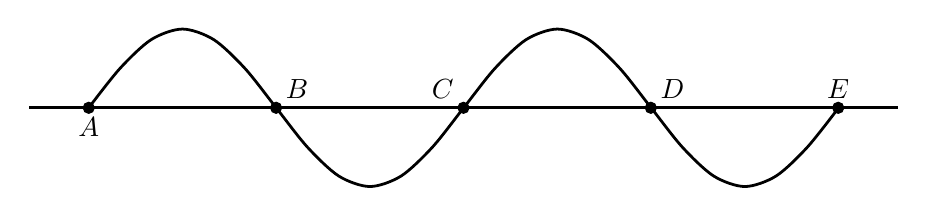
\begin{tikzpicture}[x=0.0625\textwidth]
        %% Graph
        \draw[domain=0:4*pi,smooth,line width=1pt] plot (\x, {sin(\x r)});
        \draw[black,line width=1pt] (-1,0) to (13.56,0);
        %% Labels
        \node[anchor=north]      at (0,0)    {$A$};
            \draw[fill] (0,0) circle [radius=2pt];
        \node[anchor=south west] at (3.14,0) {$B$};
            \draw[fill] (3.14,0) circle [radius=2pt];
        \node[anchor=south east] at (6.28,0) {$C$};
            \draw[fill] (6.28,0) circle [radius=2pt];
        \node[anchor=south west] at (9.42,0) {$D$};
            \draw[fill] (9.42,0) circle [radius=2pt];
        \node[anchor=south]      at (12.56,0){$E$};
            \draw[fill] (12.56,0) circle [radius=2pt];
    \end{tikzpicture}
    \end{center}
    One cycle of the motion is represented by the distance from:
    \begin{multicols}{2}
    \begin{choices}
      \correctchoice{$A$ to $B$}
        \wrongchoice{$B$ to $D$}
        \wrongchoice{$B$ to $E$}
        \wrongchoice{$A$ to $E$}
    \end{choices}
    \end{multicols}
\end{question}
}

\element{cpo-mc}{
\begin{question}{cpo-ch19-q16}
    A graph of harmonic motion shows that a cycle lasts \SI{8.0}{\second}.
    What is the frequency of this oscillator?
    \begin{multicols}{2}
    \begin{choices}
      \correctchoice{\SI{0.125}{\hertz}}
        \wrongchoice{\SI{0.125}{\second}}
        \wrongchoice{\SI{8.0}{\hertz}}
        \wrongchoice{\SI{8.0}{\second}}
    \end{choices}
    \end{multicols}
\end{question}
}

\element{cpo-mc}{
\begin{question}{cpo-ch19-q17}
    The period of a pendulum multiplied by its frequency ($T\times f$) equals:
    \begin{multicols}{2}
    \begin{choices}
        \wrongchoice{one amplitude}
        \wrongchoice{one cycle}
      \correctchoice{the number one}
        \wrongchoice{one swing}
    \end{choices}
    \end{multicols}
\end{question}
}

\element{cpo-mc}{
\begin{question}{cpo-ch19-q18}
    Assuming that it takes exactly \SI{24}{\hour} for Earth to rotate on its axis,
        the frequency of rotation for Earth is:
    \begin{multicols}{2}
    \begin{choices}
        %% NOTE: This was originally incorrect
        %\wrongchoice{\SI{0.125}{\second}}
        \wrongchoice{\SI{0.042}{\hertz}}
      \correctchoice{\SI{1.16e-5}{\hertz}}
        \wrongchoice{\SI{1400}{\hertz}}
        \wrongchoice{\SI{86000}{\hertz}}
    \end{choices}
    \end{multicols}
\end{question}
}

\element{cpo-mc}{
\begin{question}{cpo-ch19-q19}
    The unit most frequently used to measure the phase relationship between parts of the cycle of an oscillator is the:
    \begin{multicols}{2}
    \begin{choices}
        \wrongchoice{hertz (\si{\hertz})}
        \wrongchoice{meter (\si{\meter})}
      \correctchoice{degree (\si{\degree})}
        \wrongchoice{second (\si{\second})}
    \end{choices}
    \end{multicols}
\end{question}
}

\element{cpo-mc}{
\begin{question}{cpo-ch19-q20}
    One full cycle of harmonic motion is represented by:
    \begin{multicols}{4}
    \begin{choices}
        \wrongchoice{\ang{45}}
        \wrongchoice{\ang{90}}
        \wrongchoice{\ang{180}}
      \correctchoice{\ang{360}}
    \end{choices}
    \end{multicols}
\end{question}
}

\element{cpo-mc}{
\begin{question}{cpo-ch19-q21}
    Two oscillators that are \ang{180} out of phase are:
    \begin{choices}
        \wrongchoice{one-quarter of a cycle apart.}
      \correctchoice{one-half of a cycle apart.}
        \wrongchoice{three-quarters of a cycle apart.}
        \wrongchoice{one full cycle apart.}
    \end{choices}
\end{question}
}

\element{cpo-mc}{
\begin{question}{cpo-ch19-q22}
    The graph below represents position versus time for the amplitude of a pendulum that was allowed to swing for \SI{4}{\second}.
    \begin{center}
    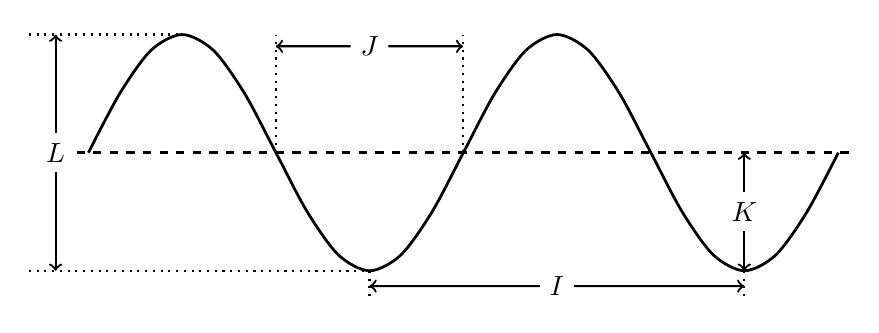
\begin{tikzpicture}[x=0.0625\textwidth,yscale=1.5]
        %% Graph
        \draw[domain=0:4*pi,smooth,line width=1pt] plot (\x, {sin(\x r)});
        \draw[dashed,line width=1pt] (-0.20,0) to (12.76,0);
        %% A Label
        \draw[thick,dotted] (-1.00,1) to (1.57,1);
        \draw[thick,dotted] (-1.00,-1) to (4.71,-1);
        \node[anchor=center] (A) at (-0.55,0) {$L$};
        \draw[thick,->] (A) to (-0.55,1);
        \draw[thick,->] (A) to (-0.55,-1);
        %% B Label
        \node[anchor=center] (B) at (10.99,-0.5) {$K$};
        \draw[thick,->] (B) to (10.99,0);
        \draw[thick,->] (B) to (10.99,-1);
        %% C Label
        \draw[thick,dotted] (3.14,0) to (3.14,1);
        \draw[thick,dotted] (6.28,0) to (6.28,1);
        \node[anchor=center] (C) at (4.71,0.9) {$J$};
        \draw[thick,->] (C) to (3.14,0.9);
        \draw[thick,->] (C) to (6.28,0.9);
        %% D Label
        \draw[thick,dotted] (4.71,-1) to (4.71,-1.25);
        \draw[thick,dotted] (10.99,-1) to (10.99,-1.25);
        \node[anchor=center] (D) at (7.85,-1.13) {$I$};
        \draw[thick,->] (D) to (4.71,-1.13);
        \draw[thick,->] (D) to (10.99,-1.13);
    \end{tikzpicture}
    \end{center}
    Which letter correctly identifies the amplitude of the pendulum?
    \begin{multicols}{4}
    \begin{choices}
        \wrongchoice{$I$}
        \wrongchoice{$J$}
      \correctchoice{$K$}
        \wrongchoice{$L$}
    \end{choices}
    \end{multicols}
\end{question}
}

\element{cpo-mc}{
\begin{question}{cpo-ch19-q23}
    The diagram below represents a segment of a periodic wave:
    \begin{center}
    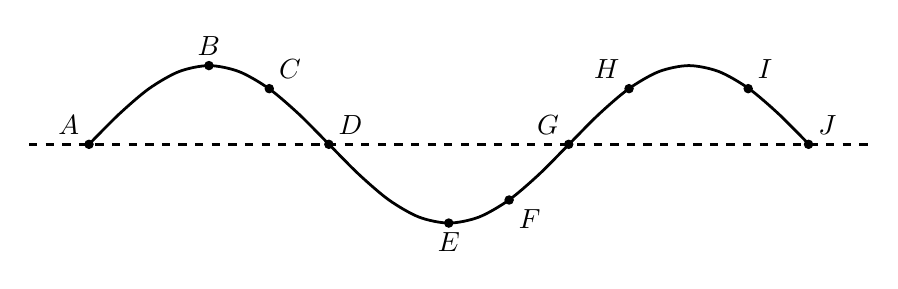
\begin{tikzpicture}[x=0.08\columnwidth]
        %% Graph
        \draw[domain=0:3*pi,smooth,line width=1pt] plot (\x, {sin(\x r)});
        \draw[dashed,line width=1pt] (-0.785,0) to (10.21,0);
        %% Labels
        \node[anchor=south east] at (0,0)    {$A$};
            \draw[fill] (0,0) circle [radius=1.5pt];
        \node[anchor=south]      at (1.57,1) {$B$};
            \draw[fill] (1.57,1) circle [radius=1.5pt];
        \node[anchor=south west] at (2.36,0.707) {$C$};
            \draw[fill] (2.36,0.707) circle [radius=1.5pt];
        \node[anchor=south west] at (3.14,0) {$D$};
            \draw[fill] (3.14,0) circle [radius=1.5pt];
        \node[anchor=north]      at (4.71,-1) {$E$};
            \draw[fill] (4.71,-1) circle [radius=1.5pt];
        \node[anchor=north west] at (5.50,-0.707) {$F$};
            \draw[fill] (5.50,-0.707) circle [radius=1.5pt];
        \node[anchor=south east] at (6.28,0) {$G$};
            \draw[fill] (6.28,0) circle [radius=1.5pt];
        \node[anchor=south east] at (7.07,0.707) {$H$};
            \draw[fill] (7.07,0.707) circle [radius=1.5pt];
        \node[anchor=south west] at (8.63,0.707) {$I$};
            \draw[fill] (8.63,0.707) circle [radius=1.5pt];
        \node[anchor=south west] at (9.42,0) {$J$};
            \draw[fill] (9.42,0) circle [radius=1.5pt];
    \end{tikzpicture}
    \end{center}
    Which two points represents the same point in a cycle?
    \begin{multicols}{2}
    \begin{choices}
      \correctchoice{$C$ and $I$}
        \wrongchoice{$A$ and $D$}
        \wrongchoice{$B$ and $E$}
        \wrongchoice{$C$ and $H$}
    \end{choices}
    \end{multicols}
\end{question}
}

\element{cpo-mc}{
\begin{question}{cpo-ch19-q24}
    One cycle of harmonic motion for a certain spring takes \SI{6}{\second}.
    If a second, identical spring is set in motion \SI{4}{\second} after the first,
        the phase relationship between the motion of the two springs differs by:
    \begin{multicols}{4}
    \begin{choices}
        \wrongchoice{\ang{67}}
        \wrongchoice{\ang{75}}
      \correctchoice{\ang{240}}
        \wrongchoice{\ang{270}}
    \end{choices}
    \end{multicols}
\end{question}
}

\element{cpo-mc}{
\begin{question}{cpo-ch19-q25}
    The diagram represents the harmonic motion of two identical,
        vibrating springs:
    \begin{center}
    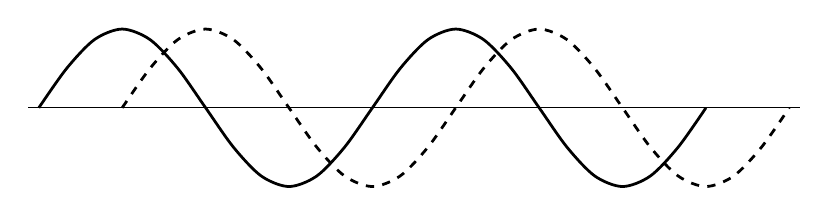
\begin{tikzpicture}[x=0.0556\columnwidth]
        %% Graph
        \draw[very thick,dashed,domain=0:4*pi,smooth,line width=1pt] plot (\x, {sin(\x r)});
        \draw[very thick,domain=0:4*pi,smooth,line width=1pt] plot (\x-1.57, {sin(\x r)});
        \draw[black] (-1.77,0) to (12.76,0);
    \end{tikzpicture}
    \end{center}
    The phase relationship of the two springs differs by approximately:
    \begin{multicols}{4}
    \begin{choices}
      \correctchoice{\ang{90}}
        \wrongchoice{\ang{180}}
        \wrongchoice{\ang{270}}
        \wrongchoice{\ang{360}}
    \end{choices}
    \end{multicols}
\end{question}
}

\element{cpo-mc}{
\begin{question}{cpo-ch19-q26}
    Resonance occurs for a system in harmonic motion when the:
    \begin{choices}
        \wrongchoice{frequency of the periodic force is larger than the natural frequency of the system.}
      \correctchoice{frequency of the periodic force equals than the natural frequency of the system.}
        \wrongchoice{frequency of the periodic force is less than the natural frequency of the system.}
        \wrongchoice{Resonance cannot occur for a system in harmonic motion.}
    \end{choices}
\end{question}
}

\element{cpo-mc}{
\begin{question}{cpo-ch19-q27}
    If you triple the mass on a pendulum bob,
        the period of the pendulum:
    \begin{choices}
        \wrongchoice{increases by \num{3} times}
        \wrongchoice{decreases by \num{1/3}}
      \correctchoice{does not change}
        \wrongchoice{increases by \num{1/3}}
    \end{choices}
\end{question}
}

\element{cpo-mc}{
\begin{question}{cpo-ch19-q28}
    The force that brings the motion of an oscillator toward its equilibrium position is called its:
    \begin{multicols}{2}
    \begin{choices}
        \wrongchoice{gravitational force}
        \wrongchoice{strong force}
      \correctchoice{restoring force}
        \wrongchoice{centripetal force}
    \end{choices}
    \end{multicols}
\end{question}
}

\element{cpo-mc}{
\begin{question}{cpo-ch19-q29}
    You can change the natural frequency of a pendulum by changing the:
    \begin{choices}
        \wrongchoice{mass of the pendulum bob.}
      \correctchoice{length of the pendulum string.}
        \wrongchoice{amplitude of the restoring force.}
        \wrongchoice{The natural frequency of a pendulum cannot be changed.}
    \end{choices}
\end{question}
}

\element{cpo-mc}{
\begin{question}{cpo-ch19-q30}
    As an oscillating spring is moved farther from its equilibrium position, the:
    \begin{choices}
      \correctchoice{energy does not change.}
        \wrongchoice{amplitude decreases.}
        \wrongchoice{period increases.}
        \wrongchoice{restoring force increases.}
    \end{choices}
\end{question}
}


\endinput


